% Options for packages loaded elsewhere
\PassOptionsToPackage{unicode}{hyperref}
\PassOptionsToPackage{hyphens}{url}
\PassOptionsToPackage{dvipsnames,svgnames*,x11names*}{xcolor}
%
\documentclass[
  8pt,
  ignorenonframetext,
  dvipsnames]{beamer}
\usepackage{pgfpages}
\setbeamertemplate{caption}[numbered]
\setbeamertemplate{caption label separator}{: }
\setbeamercolor{caption name}{fg=normal text.fg}
\beamertemplatenavigationsymbolsempty
% Prevent slide breaks in the middle of a paragraph
\widowpenalties 1 10000
\raggedbottom
\setbeamertemplate{part page}{
  \centering
  \begin{beamercolorbox}[sep=16pt,center]{part title}
    \usebeamerfont{part title}\insertpart\par
  \end{beamercolorbox}
}
\setbeamertemplate{section page}{
  \centering
  \begin{beamercolorbox}[sep=12pt,center]{part title}
    \usebeamerfont{section title}\insertsection\par
  \end{beamercolorbox}
}
\setbeamertemplate{subsection page}{
  \centering
  \begin{beamercolorbox}[sep=8pt,center]{part title}
    \usebeamerfont{subsection title}\insertsubsection\par
  \end{beamercolorbox}
}
\AtBeginPart{
  \frame{\partpage}
}
\AtBeginSection{
  \ifbibliography
  \else
    \frame{\sectionpage}
  \fi
}
\AtBeginSubsection{
  \frame{\subsectionpage}
}
\usepackage{amsmath,amssymb}
\usepackage{lmodern}
\usepackage{ifxetex,ifluatex}
\ifnum 0\ifxetex 1\fi\ifluatex 1\fi=0 % if pdftex
  \usepackage[T1]{fontenc}
  \usepackage[utf8]{inputenc}
  \usepackage{textcomp} % provide euro and other symbols
\else % if luatex or xetex
  \usepackage{unicode-math}
  \defaultfontfeatures{Scale=MatchLowercase}
  \defaultfontfeatures[\rmfamily]{Ligatures=TeX,Scale=1}
\fi
% Use upquote if available, for straight quotes in verbatim environments
\IfFileExists{upquote.sty}{\usepackage{upquote}}{}
\IfFileExists{microtype.sty}{% use microtype if available
  \usepackage[]{microtype}
  \UseMicrotypeSet[protrusion]{basicmath} % disable protrusion for tt fonts
}{}
\makeatletter
\@ifundefined{KOMAClassName}{% if non-KOMA class
  \IfFileExists{parskip.sty}{%
    \usepackage{parskip}
  }{% else
    \setlength{\parindent}{0pt}
    \setlength{\parskip}{6pt plus 2pt minus 1pt}}
}{% if KOMA class
  \KOMAoptions{parskip=half}}
\makeatother
\usepackage{xcolor}
\IfFileExists{xurl.sty}{\usepackage{xurl}}{} % add URL line breaks if available
\IfFileExists{bookmark.sty}{\usepackage{bookmark}}{\usepackage{hyperref}}
\hypersetup{
  pdftitle={Data Analysis for Policy Research Using R},
  pdfauthor={Harold Stolper},
  colorlinks=true,
  linkcolor=Maroon,
  filecolor=Maroon,
  citecolor=Blue,
  urlcolor=blue,
  pdfcreator={LaTeX via pandoc}}
\urlstyle{same} % disable monospaced font for URLs
\newif\ifbibliography
\usepackage{color}
\usepackage{fancyvrb}
\newcommand{\VerbBar}{|}
\newcommand{\VERB}{\Verb[commandchars=\\\{\}]}
\DefineVerbatimEnvironment{Highlighting}{Verbatim}{commandchars=\\\{\}}
% Add ',fontsize=\small' for more characters per line
\usepackage{framed}
\definecolor{shadecolor}{RGB}{248,248,248}
\newenvironment{Shaded}{\begin{snugshade}}{\end{snugshade}}
\newcommand{\AlertTok}[1]{\textcolor[rgb]{0.94,0.16,0.16}{#1}}
\newcommand{\AnnotationTok}[1]{\textcolor[rgb]{0.56,0.35,0.01}{\textbf{\textit{#1}}}}
\newcommand{\AttributeTok}[1]{\textcolor[rgb]{0.77,0.63,0.00}{#1}}
\newcommand{\BaseNTok}[1]{\textcolor[rgb]{0.00,0.00,0.81}{#1}}
\newcommand{\BuiltInTok}[1]{#1}
\newcommand{\CharTok}[1]{\textcolor[rgb]{0.31,0.60,0.02}{#1}}
\newcommand{\CommentTok}[1]{\textcolor[rgb]{0.56,0.35,0.01}{\textit{#1}}}
\newcommand{\CommentVarTok}[1]{\textcolor[rgb]{0.56,0.35,0.01}{\textbf{\textit{#1}}}}
\newcommand{\ConstantTok}[1]{\textcolor[rgb]{0.00,0.00,0.00}{#1}}
\newcommand{\ControlFlowTok}[1]{\textcolor[rgb]{0.13,0.29,0.53}{\textbf{#1}}}
\newcommand{\DataTypeTok}[1]{\textcolor[rgb]{0.13,0.29,0.53}{#1}}
\newcommand{\DecValTok}[1]{\textcolor[rgb]{0.00,0.00,0.81}{#1}}
\newcommand{\DocumentationTok}[1]{\textcolor[rgb]{0.56,0.35,0.01}{\textbf{\textit{#1}}}}
\newcommand{\ErrorTok}[1]{\textcolor[rgb]{0.64,0.00,0.00}{\textbf{#1}}}
\newcommand{\ExtensionTok}[1]{#1}
\newcommand{\FloatTok}[1]{\textcolor[rgb]{0.00,0.00,0.81}{#1}}
\newcommand{\FunctionTok}[1]{\textcolor[rgb]{0.00,0.00,0.00}{#1}}
\newcommand{\ImportTok}[1]{#1}
\newcommand{\InformationTok}[1]{\textcolor[rgb]{0.56,0.35,0.01}{\textbf{\textit{#1}}}}
\newcommand{\KeywordTok}[1]{\textcolor[rgb]{0.13,0.29,0.53}{\textbf{#1}}}
\newcommand{\NormalTok}[1]{#1}
\newcommand{\OperatorTok}[1]{\textcolor[rgb]{0.81,0.36,0.00}{\textbf{#1}}}
\newcommand{\OtherTok}[1]{\textcolor[rgb]{0.56,0.35,0.01}{#1}}
\newcommand{\PreprocessorTok}[1]{\textcolor[rgb]{0.56,0.35,0.01}{\textit{#1}}}
\newcommand{\RegionMarkerTok}[1]{#1}
\newcommand{\SpecialCharTok}[1]{\textcolor[rgb]{0.00,0.00,0.00}{#1}}
\newcommand{\SpecialStringTok}[1]{\textcolor[rgb]{0.31,0.60,0.02}{#1}}
\newcommand{\StringTok}[1]{\textcolor[rgb]{0.31,0.60,0.02}{#1}}
\newcommand{\VariableTok}[1]{\textcolor[rgb]{0.00,0.00,0.00}{#1}}
\newcommand{\VerbatimStringTok}[1]{\textcolor[rgb]{0.31,0.60,0.02}{#1}}
\newcommand{\WarningTok}[1]{\textcolor[rgb]{0.56,0.35,0.01}{\textbf{\textit{#1}}}}
\usepackage{longtable,booktabs,array}
\usepackage{calc} % for calculating minipage widths
\usepackage{caption}
% Make caption package work with longtable
\makeatletter
\def\fnum@table{\tablename~\thetable}
\makeatother
\usepackage{graphicx}
\makeatletter
\def\maxwidth{\ifdim\Gin@nat@width>\linewidth\linewidth\else\Gin@nat@width\fi}
\def\maxheight{\ifdim\Gin@nat@height>\textheight\textheight\else\Gin@nat@height\fi}
\makeatother
% Scale images if necessary, so that they will not overflow the page
% margins by default, and it is still possible to overwrite the defaults
% using explicit options in \includegraphics[width, height, ...]{}
\setkeys{Gin}{width=\maxwidth,height=\maxheight,keepaspectratio}
% Set default figure placement to htbp
\makeatletter
\def\fps@figure{htbp}
\makeatother
\setlength{\emergencystretch}{3em} % prevent overfull lines
\providecommand{\tightlist}{%
  \setlength{\itemsep}{0pt}\setlength{\parskip}{0pt}}
\setcounter{secnumdepth}{-\maxdimen} % remove section numbering

%packages
\usepackage{graphicx}
\usepackage{rotating}
\usepackage{hyperref}

\usepackage{tikz} % used for text highlighting, amongst others
\usepackage{comment}

%title slide stuff
%\institute{Department of Education}
%\title{Managing and Manipulating Data Using R}

%
\setbeamertemplate{navigation symbols}{} % get rid of navigation icons:
\setbeamertemplate{footline}[page number]

%\setbeamertemplate{frametitle}{\thesection \hspace{0.2cm} \insertframetitle}
\setbeamertemplate{section in toc}[sections numbered]
%\setbeamertemplate{subsection in toc}[subsections numbered]
\setbeamertemplate{subsection in toc}{%
  \leavevmode\leftskip=3.2em\color{gray}\rlap{\hskip-2em\inserttocsectionnumber.\inserttocsubsectionnumber}\inserttocsubsection\par
}

%define colors
%\definecolor{uva_orange}{RGB}{216,141,42} % UVa orange (Rotunda orange)
\definecolor{mygray}{rgb}{0.95, 0.95, 0.95} % for highlighted text
	% grey is equal parts red, green, blue. higher values >> lighter grey
	%\definecolor{lightgraybo}{rgb}{0.83, 0.83, 0.83}

% new commands

%highlight text with very light grey
\newcommand*{\hlg}[1]{%
	\tikz[baseline=(X.base)] \node[rectangle, fill=mygray] (X) {#1};%
}
%, inner sep=0.3mm
%highlight text with very light grey and use font associated with code
\newcommand*{\hlgc}[1]{\texttt{\hlg{#1}}}

%modifying back ticks to add grey background
\let\OldTexttt\texttt
\renewcommand{\texttt}[1]{\OldTexttt{\hlg{#1}}}


\begin{comment}

% Font
\usepackage[defaultfam,light,tabular,lining]{montserrat}
\usepackage[T1]{fontenc}
\renewcommand*\oldstylenums[1]{{\fontfamily{Montserrat-TOsF}\selectfont #1}}

% Change color of boldface text to darkgray
\renewcommand{\textbf}[1]{{\color{darkgray}\bfseries\fontfamily{Montserrat-TOsF}#1}}

% Bullet points
\setbeamertemplate{itemize item}{\color{BlueViolet}$\circ$}
\setbeamertemplate{itemize subitem}{\color{BrickRed}$\triangleright$}
\setbeamertemplate{itemize subsubitem}{$-$}

% Reduce space before lists
%\addtobeamertemplate{itemize/enumerate body begin}{}{\vspace*{-8pt}}

\let\olditem\item
\renewcommand{\item}{%
  \olditem\vspace{4pt}
}

% decreasing space before and after level-2 bullet block
%\addtobeamertemplate{itemize/enumerate subbody begin}{}{\vspace*{-3pt}}
%\addtobeamertemplate{itemize/enumerate subbody end}{}{\vspace*{-3pt}}

% decreasing space before and after level-3 bullet block
%\addtobeamertemplate{itemize/enumerate subsubbody begin}{}{\vspace*{-2pt}}
%\addtobeamertemplate{itemize/enumerate subsubbody end}{}{\vspace*{-2pt}}

%Section numbering
\setbeamertemplate{section page}{%
    \begingroup
        \begin{beamercolorbox}[sep=10pt,center,rounded=true,shadow=true]{section title}
        \usebeamerfont{section title}\thesection~\insertsection\par
        \end{beamercolorbox}
    \endgroup
}

\setbeamertemplate{subsection page}{%
    \begingroup
        \begin{beamercolorbox}[sep=6pt,center,rounded=true,shadow=true]{subsection title}
        \usebeamerfont{subsection title}\thesection.\thesubsection~\insertsubsection\par
        \end{beamercolorbox}
    \endgroup
}

\end{comment}
\ifluatex
  \usepackage{selnolig}  % disable illegal ligatures
\fi

\title{Data Analysis for Policy Research Using R}
\subtitle{Introduction and R Basics}
\author{Harold Stolper}
\date{}

\begin{document}
\frame{\titlepage}

\begin{frame}[allowframebreaks]
  \tableofcontents[hideallsubsections]
\end{frame}
\hypertarget{introductions}{%
\section{Introductions}\label{introductions}}

\begin{frame}{Student introductions}
\protect\hypertarget{student-introductions}{}
\begin{enumerate}
\tightlist
\item
  Preferred name
\item
  Pronouns (if comfortable)
\item
  Previous R exposure/experience
\item
  And answer one of these two questions:

  \begin{itemize}
  \tightlist
  \item
    What's something you would eventually like to learn how to do in R?
  \item
    What's something that you have observed or think is important that
    people in your field aren't paying attention to?
  \end{itemize}
\item
  (optional) One piece of culture you are excited about right now

  \begin{itemize}
  \tightlist
  \item
    e.g.~music, writing, fashion, a meme, other art, sports, etc.
  \end{itemize}
\end{enumerate}
\end{frame}

\begin{frame}{Teaching Assistants}
\protect\hypertarget{teaching-assistants}{}
\begin{itemize}
\tightlist
\item
  Liam Tay Kearney (morning section)
\item
  Sasha Foster-Andres (afternoon section)
\end{itemize}
\end{frame}

\begin{frame}{Harold Stolper, instructor}
\protect\hypertarget{harold-stolper-instructor}{}
Graduated from SIPA many moons ago, returned to Columbia for my PhD in
economics.

\medskip

Recent background:

\begin{itemize}
\tightlist
\item
  This is my 7th year teaching quant courses at SIPA.
\item
  Worked as the economist for a non-profit doing research and advocacy
  to promote upward mobility for low-income NYers.
\item
  Recent focus on documenting racist police enforcement of fare evasion,
  and other topics related to policing, neighborhood change, and transit
  accessibility.
\end{itemize}

\medskip

Transitioned from Stata to R after years of using and teaching Stata.
\end{frame}

\hypertarget{what-is-r-and-how-will-we-use-it}{%
\section{What is R and How Will We Use
It?}\label{what-is-r-and-how-will-we-use-it}}

\begin{frame}{What is R?}
\protect\hypertarget{what-is-r}{}
\begin{itemize}
\tightlist
\item
  R is ``an alternative to traditional statistical packages such as
  SPSS, SAS, and Stata such that it is an extensible, open-source
  language and computing environment for Windows, Macintosh, UNIX, and
  Linux platforms.''
  \href{https://www.icpsr.umich.edu/icpsrweb/content/shared/ICPSR/faqs/what-is-r.html}{(ICPSR)}
\end{itemize}

\medskip

\begin{itemize}
\tightlist
\item
  ``R is an integrated suite of software facilities for data
  manipulation, calculation and graphical display.''
  (\href{https://www.r-project.org/about.html}{R-project.org})
\end{itemize}
\end{frame}

\begin{frame}{How will we use R?}
\protect\hypertarget{how-will-we-use-r}{}
\begin{itemize}
\tightlist
\item
  \href{https://www.rstudio.com/products/rstudio/download/preview}{RStudio}
  is a powerful user interface for R.

  \begin{itemize}
  \tightlist
  \item
    After installing R and RStudio, we'll be working entirely in the
    RStudio interface.
  \item
    We'll be working with R scripts every week! (an R script is more or
    less a text file that RStudio recognizes as R code)
  \end{itemize}
\end{itemize}

\medskip

\begin{itemize}
\tightlist
\item
  \href{https://rmarkdown.rstudio.com/lesson-1.html}{R Markdown} files
  are used in RStudio to ``both save and execute code generate high
  quality reports that can be shared with an audience.''

  \begin{itemize}
  \tightlist
  \item
    This lecture was created using R Markdown.
  \item
    Beginning next week, everything you \emph{submit} for this class
    will be a document generated with R Markdown.
  \item
    But you're workflow should always begin with an R script before
    writing up your work using R Markdown
  \end{itemize}
\end{itemize}
\end{frame}

\begin{frame}[fragile]{Base R vs.~user-defined R packages}
\protect\hypertarget{base-r-vs.-user-defined-r-packages}{}
R uses ``packages'' as a bundle of code, data and documentation.

There are default
\href{https://stat.ethz.ch/R-manual/R-devel/library/base/html/00Index.html}{base
packages} that come with R. Some examples:

\begin{itemize}
\tightlist
\item
  \texttt{base}~\\
\item
  \texttt{stats}~\\
\item
  \texttt{utils}
\end{itemize}

And there are \href{http://r-pkgs.had.co.nz/intro.html}{R packages}
developed and shared by others. Some R packages include:

\begin{itemize}
\tightlist
\item
  \texttt{tidyverse}~\\
\item
  \texttt{ggplot2}
\end{itemize}

More about these in later weeks\ldots{}
\end{frame}

\begin{frame}[fragile]{Installing and loading R packages}
\protect\hypertarget{installing-and-loading-r-packages}{}
You only need to install a package once. To install an R package use
\texttt{install.package()} function.

\begin{Shaded}
\begin{Highlighting}[]
\FunctionTok{install.packages}\NormalTok{(}\StringTok{"tidyverse"}\NormalTok{)}
\end{Highlighting}
\end{Shaded}

But you need to load a package every time you open R using the
\texttt{library()} function.

\begin{Shaded}
\begin{Highlighting}[]
\FunctionTok{library}\NormalTok{(tidyverse)}
\CommentTok{\#\textgreater{} {-}{-} Attaching packages {-}{-}{-}{-}{-}{-}{-}{-}{-}{-}{-}{-}{-}{-}{-}{-}{-}{-}{-}{-}{-}{-}{-}{-}{-}{-}{-}{-}{-}{-}{-}{-}{-}{-}{-}{-}{-}{-}{-} tidyverse 1.3.1 {-}{-}}
\CommentTok{\#\textgreater{} v ggplot2 3.3.5     v purrr   0.3.4}
\CommentTok{\#\textgreater{} v tibble  3.1.3     v dplyr   1.0.7}
\CommentTok{\#\textgreater{} v tidyr   1.1.3     v stringr 1.4.0}
\CommentTok{\#\textgreater{} v readr   2.0.0     v forcats 0.5.1}
\CommentTok{\#\textgreater{} {-}{-} Conflicts {-}{-}{-}{-}{-}{-}{-}{-}{-}{-}{-}{-}{-}{-}{-}{-}{-}{-}{-}{-}{-}{-}{-}{-}{-}{-}{-}{-}{-}{-}{-}{-}{-}{-}{-}{-}{-}{-}{-}{-}{-}{-} tidyverse\_conflicts() {-}{-}}
\CommentTok{\#\textgreater{} x dplyr::filter() masks stats::filter()}
\CommentTok{\#\textgreater{} x dplyr::lag()    masks stats::lag()}
\end{Highlighting}
\end{Shaded}
\end{frame}

\begin{frame}{What can you do with R+RStudio+RMarkdown?}
\protect\hypertarget{what-can-you-do-with-rrstudiormarkdown}{}
Things you can also do using Stata:

\begin{itemize}
\tightlist
\item
  Data cleaning and manipulation
\item
  Statistical analysis and plots
\end{itemize}

\medskip

Things you generally can't do in Stata:

\begin{itemize}
\tightlist
\item
  Generate reports and presentations
\item
  Generate interactive content

  \begin{itemize}
  \tightlist
  \item
    Maps
  \item
    Graphs
  \item
    Dashboards
  \end{itemize}
\end{itemize}
\end{frame}

\begin{frame}{What will we be doing in this class?}
\protect\hypertarget{what-will-we-be-doing-in-this-class}{}
We'll be learning how to use R to explore data to inform policy.

That means we'll be spending a lot of time working through R, but also
thinking about how/when to use the methods and concepts we've learned in
Quant I and II:

\begin{itemize}
\item
  \textbf{Research design:} understanding how data structure and methods
  impact analysis and causal inference
\item
  \textbf{Data wrangling:} cleaning and structuring messy data for
  analysis
\item
  \textbf{Exploratory analysis:} identifying and analyzing key factors
  in your analysis
\item
  \textbf{Explanatory analysis:} estimating relationships between
  variables to inform policy
\item
  \textbf{Data visualization \& presentation:} conveying findings to
  your target audience
\item
  \textbf{Policy writing \& interpretation:} translating statistical
  analysis in accessible terms
\item
  \textbf{Data advocacy}: thinking critically about using \emph{data for
  good}
\end{itemize}
\end{frame}

\begin{frame}{Examples from student project work}
\protect\hypertarget{examples-from-student-project-work}{}
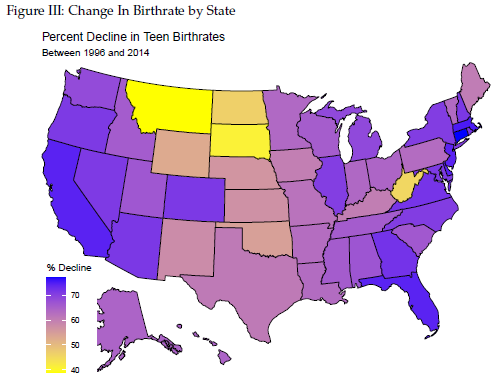
\includegraphics{lo_jo_map1.png}
\end{frame}

\begin{frame}{Examples from student project work}
\protect\hypertarget{examples-from-student-project-work-1}{}
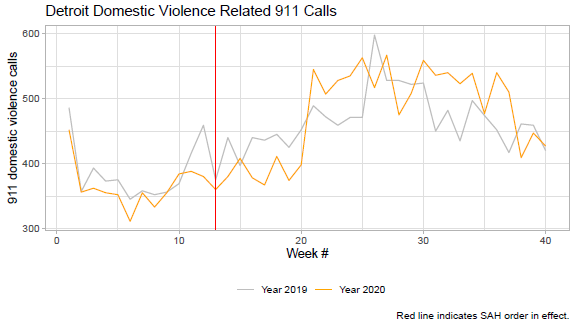
\includegraphics{nm-ca_chart1.png}
\end{frame}

\begin{frame}{Examples from student project work}
\protect\hypertarget{examples-from-student-project-work-2}{}
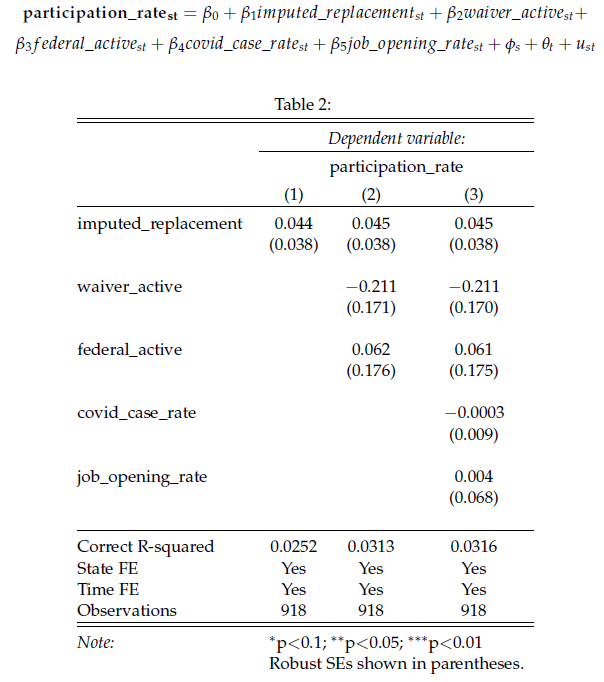
\includegraphics[width=0.6\textwidth,height=\textheight]{ps_ra_regtable.png}
\end{frame}

\hypertarget{prerequisites-r-setup-course-goals}{%
\section{Prerequisites, R setup, course
goals}\label{prerequisites-r-setup-course-goals}}

\begin{frame}{Questions for you}
\protect\hypertarget{questions-for-you}{}
\url{https://pollev.com/haroldpoll}
\end{frame}

\hypertarget{r-projects-and-directory-structure}{%
\section{R Projects and Directory
Structure}\label{r-projects-and-directory-structure}}

\begin{frame}[fragile]{Working directory}
\protect\hypertarget{working-directory}{}
R looks for files in your \textbf{working directory}

Function \texttt{getwd()} shows the current working directory (also
shown at the top of the RStudio console.)

\begin{Shaded}
\begin{Highlighting}[]
\FunctionTok{getwd}\NormalTok{()}
\CommentTok{\#\textgreater{} [1] "C:/Users/hstol/My Drive/SIPA/R {-} Data Analysis/U6614/Lectures/Lecture1"}
\end{Highlighting}
\end{Shaded}

You can see all files located in your working directory in the
``Files/Plots/Packages/ Help/Viewer'' pane (by default in the lower
right)
\end{frame}

\begin{frame}{RStudio
\href{https://bookdown.org/ndphillips/YaRrr/the-four-rstudio-windows.html}{interface}}
\protect\hypertarget{rstudio-interface}{}
\includegraphics{rstudio_session_4pane_layout.png}
\end{frame}

\begin{frame}[fragile]{So what is the working directory?}
\protect\hypertarget{so-what-is-the-working-directory}{}
When you run code from the \textbf{R Console} or an \textbf{R Script},
or from \textbf{code chunks} in an RMarkdown file (.rmd), the working
directory is\ldots{}

\begin{itemize}
\tightlist
\item
  the folder your file is saved in, or \ldots{}
\item
  if you are working within an \textbf{R Project}, the working directory
  is the main directory for the project (more on that shortly!)
\end{itemize}

\begin{Shaded}
\begin{Highlighting}[]
\FunctionTok{getwd}\NormalTok{()}
\CommentTok{\#\textgreater{} [1] "C:/Users/hstol/My Drive/SIPA/R {-} Data Analysis/U6614/Lectures/Lecture1"}
\end{Highlighting}
\end{Shaded}

\begin{itemize}
\tightlist
\item
  For this class we'll be using R projects to keep organized.
\end{itemize}
\end{frame}

\begin{frame}{What is an R project? Why are we using them?}
\protect\hypertarget{what-is-an-r-project-why-are-we-using-them}{}
What is an ``R project''?

\begin{itemize}
\tightlist
\item
  A file that keeps all ``project'' files organized together: -- input
  data, R scripts, analytical results, and figures.
\item
  When you open an R project, your working directory is automatically
  set to the directory where your R project (and related files) lives.
\end{itemize}

Why will we be asking you to create and work with R projects?

\begin{itemize}
\tightlist
\item
  Projects are important for keeping organized and avoiding file path
  errors
\item
  You should have a project for every week that will include R scripts
  from class, data files, and also R Markdown files that you'll create
  for assignments.
\item
  We also want you to be able to run the R Markdown files (.rmd) used to
  generate each lecture.

  \begin{itemize}
  \tightlist
  \item
    You can create or download an R project with directory structure
    (i.e.~organizing files and sub-folders in a particular way) to
    recreate course documents on your own.
  \end{itemize}
\end{itemize}
\end{frame}

\begin{frame}[fragile]{The path is how we refer to a directory}
\protect\hypertarget{the-path-is-how-we-refer-to-a-directory}{}
\textbf{Absolute file path}: a complete list of directories needed to
locate a file or folder.

\smallskip

\texttt{setwd("C:/Users/Harold\ Stolper/Google\ Drive/SIPA/R\ -\ Data\ Analysis/Fall\ 2020/Lectures/Lecture\ 1")}

\medskip

\textbf{Relative file path}: a way of indicating a given file location
relative to your working directory (note that they might be the same!)

\begin{itemize}
\tightlist
\item
  Assuming your current working directory is in the ``lecture2'' folder
  and you want to go up 2 levels to the ``Fall 2021'' folder, your
  relative file path would look something like this:
\end{itemize}

\texttt{setwd("../../")}

\medskip

\textbf{File path shortcuts:}

\begin{longtable}[]{@{}ll@{}}
\toprule
\textbf{Key} & \textbf{Description} \\
\midrule
\endhead
\textasciitilde{} & tilde is a shortcut for user's home directory (mine
is my name pm) \\
../ & moves up a level \\
../../ & moves up two level \\
\bottomrule
\end{longtable}
\end{frame}

\hypertarget{r-basics}{%
\section{R Basics}\label{r-basics}}

\begin{frame}{Executing code in R}
\protect\hypertarget{executing-code-in-r}{}
Three ways to execute commands in R

\begin{enumerate}
\tightlist
\item
  \textbf{Console:} type/paste commands to run ``on the fly''
\item
  \textbf{R scripts} (.r files)

  \begin{itemize}
  \tightlist
  \item
    Just a text file full of R commands
  \item
    Can execute one command at a time, several commands at a time, or
    the entire script
  \end{itemize}
\item
  \textbf{Code chunks} in R Markdown (.rmd files)

  \begin{itemize}
  \tightlist
  \item
    Can execute one command at a time, one chunk at a time, or ``knit''
    the entire file into a document (e.g.~html or pdf)
  \end{itemize}
\end{enumerate}
\end{frame}

\begin{frame}{Shortcuts for executing commands}
\protect\hypertarget{shortcuts-for-executing-commands}{}
Three ways to execute commands in R

\begin{enumerate}
\tightlist
\item
  Type/paste commands directly into the ``console'' (and press ENTER)
\item
  R scripts (.R files)

  \begin{itemize}
  \tightlist
  \item
    \textbf{Cmd/Ctrl + Enter}: execute highlighted line(s)
  \item
    \textbf{Cmd/Ctrl + Shift + Enter} (without highlighting any lines):
    run entire script
  \end{itemize}
\item
  `code chunks' in RMarkdown (.rmd files)

  \begin{itemize}
  \tightlist
  \item
    \textbf{Cmd/Ctrl + Enter}: execute highlighted line(s) within chunk
  \item
    \textbf{Cmd/Ctrl + Shift + k}: ``knit'' entire document
  \end{itemize}
\end{enumerate}
\end{frame}

\begin{frame}[fragile]{Assignment}
\protect\hypertarget{assignment}{}
\textbf{Assignment} means assigning a value/set of values to an
``object''

\begin{itemize}
\tightlist
\item
  \texttt{\textless{}-} is the assignment operator

  \begin{itemize}
  \tightlist
  \item
    in other languages \texttt{=} is the assignment operator
  \end{itemize}
\item
  good practice to put a space before and after assignment operator
\end{itemize}

\begin{Shaded}
\begin{Highlighting}[]
\CommentTok{\# Create an object a and assign value}
\NormalTok{a }\OtherTok{\textless{}{-}} \DecValTok{5}
\NormalTok{a}
\CommentTok{\#\textgreater{} [1] 5}

\CommentTok{\# Create an object b and assign value}
\NormalTok{b }\OtherTok{\textless{}{-}} \StringTok{"I\textquotesingle{}m so excited to be on Zoom again!"}
\NormalTok{b}
\CommentTok{\#\textgreater{} [1] "I\textquotesingle{}m so excited to be on Zoom again!"}
\end{Highlighting}
\end{Shaded}

Note 1: comments start with one or more \texttt{\#} symbols

Note 2: R is caps sensitive!
\end{frame}

\begin{frame}{Objects and assignment}
\protect\hypertarget{objects-and-assignment}{}
R stores information in objects (like all ``object-oriented''
programming languages).

Some objects:

\begin{itemize}
\tightlist
\item
  numbers
\item
  character strings
\item
  vectors
\item
  matrices
\item
  lists
\item
  functions
\item
  plots
\item
  data frames (the datasets of R!)
\end{itemize}
\end{frame}

\begin{frame}{Functions}
\protect\hypertarget{functions}{}
Functions do things to different objects. They often accept arguments --
we ``pass'' arguments to functions.

Functions are also objects themselves that can be ``called'' to do
things like:

\begin{itemize}
\tightlist
\item
  calculate and display statistics
\item
  generate output
\item
  display part or all of objects (e.g.~show some data)
\item
  manipulate objects (e.g.~create a new column of data)
\item
  extract information from objects (e.g.~the number of rows of data)
\end{itemize}

Base R includes lots of functions. We'll be working with additional
packages that include some handy functions.
\end{frame}

\begin{frame}{Let's jump in!}
\protect\hypertarget{lets-jump-in}{}
Our goals for today's R workshop example are very modest:

\begin{itemize}
\tightlist
\item
  Create an R project including R script.
\item
  Look around and get our bearings.
\item
  Install and load a package
  (\href{https://www.gapminder.org/}{gapminder}).
\item
  Use base R functions to inspect a data frame included with this
  package.
\item
  Use some functions to perform some very basic analysis.
\item
  Assign results from our analysis to new objects and display them.
\end{itemize}
\end{frame}

\hypertarget{assignments-and-other-course-responsibilities}{%
\section{Assignments and other course
responsibilities}\label{assignments-and-other-course-responsibilities}}

\begin{frame}{Assignment 1: submit an R script via CW by 11:59pm next
Monday}
\protect\hypertarget{assignment-1-submit-an-r-script-via-cw-by-1159pm-next-monday}{}
Create an R script called assignment1.r that includes code and answers
(as comments) for the following:

\begin{enumerate}
\setcounter{enumi}{-1}
\tightlist
\item
  Create a new R project called assignment1.

  \begin{itemize}
  \tightlist
  \item
    This is for your internal project management, do not submit your R
    project file.
  \end{itemize}
\item
  Load the gapminder data using the library function.

  \begin{itemize}
  \tightlist
  \item
    You'll need to install the gapminder package if you didn't follow
    along in class today.
  \end{itemize}
\item
  Show the data structure of the gapminder data frame in the gapminder
  package.
\item
  What is the average gdpPercap across all observations in the data
  frame?

  \begin{itemize}
  \tightlist
  \item
    Use ?gapminder to access gapminder documentation and find the units
    for gdpPercap.
  \item
    How would you interpret this mean? i.e.~what is it the mean of?
  \end{itemize}
\item
  Plot year (x-axis) vs.~gdpPercap (y-axis).

  \begin{itemize}
  \tightlist
  \item
    Describe what the plot says about economic growth over time.
  \end{itemize}
\item
  Create a barplot showing the number of observations in each continent.

  \begin{itemize}
  \tightlist
  \item
    Start by using the table function with continents as its argument.
  \item
    Next pass the object created by this function to the barplot
    function.
  \end{itemize}
\end{enumerate}
\end{frame}

\begin{frame}{General assignment guidance}
\protect\hypertarget{general-assignment-guidance}{}
\begin{itemize}
\tightlist
\item
  Use blank spaces liberally, code is hard to read and spaces help!
\item
  Use comments liberally throughout your R script to describe your
  steps.
\item
  Troubleshooting is a skill! Here are some tips and resources:

  \begin{itemize}
  \tightlist
  \item
    Consult the R script from today's class for examples.
  \item
    Get used to using R's built in documentation by using ?
  \item
    Use Google liberally for examples that work.
  \item
    When you're stuck, focus on finding examples to get your own code to
    work, even if you don't feel comfortable with all the syntax just
    yet.
  \end{itemize}
\item
  Consulting with others is good! Copying, however, is not the way to
  learn to code.

  \begin{itemize}
  \tightlist
  \item
    \textbf{Copied assignment submissions will result in a 0 for all
    parties.}
  \end{itemize}
\end{itemize}
\end{frame}

\begin{frame}{Use Ed Discussion for help!}
\protect\hypertarget{use-ed-discussion-for-help}{}
\begin{itemize}
\tightlist
\item
  If you need help troubleshooting errors, posting to
  \href{https://edstem.org/us/courses/18438/discussion/}{Ed Discussion}
  is usually a great place to start (in addition to office hours).
\item
  Your post should provide a
  \href{https://stackoverflow.com/help/minimal-reproducible-example}{reproducible
  example}, including code and a screenshot of the output/error message
  if applicable.
\item
  Don't hesitate to post for help troubleshooting code or setup
  issues\ldots{} if you're running intro trouble, odds are somebody else
  is too!
\item
  A teaching team member will reply soon, and you are also encouraged to
  reply to each others' posts if you have insight about how to resolve
  the issue.
\end{itemize}
\end{frame}

\begin{frame}{Quizzes on pre-class lessons}
\protect\hypertarget{quizzes-on-pre-class-lessons}{}
Starting next class, every class will begin with a short Courseworks
quiz covering the pre-class lessons:

\begin{itemize}
\tightlist
\item
  Typically 10 multiple choice questions in total, \textasciitilde5
  minutes to complete
\item
  Will include 1 question on the Data Primer covering the data to be
  used next class
\end{itemize}
\end{frame}

\begin{frame}{Attendance and participation}
\protect\hypertarget{attendance-and-participation}{}
\textbf{Recitation}

\begin{itemize}
\tightlist
\item
  You must be able to attend one of the Thursday recitation times

  \begin{itemize}
  \tightlist
  \item
    Early in the semester recitation will be used to review code from
    class and prep for assignments
  \item
    Later in the semester this time will be used for extra office hours
    and project meetings
  \end{itemize}
\end{itemize}

\textbf{Zoom}

\begin{itemize}
\tightlist
\item
  After in-person instruction resumes, whenever possible Zoom links will
  be shared w/students who are feeling unwell or dealing with COVID
  related disruptions

  \begin{itemize}
  \tightlist
  \item
    To request a Zoom link, please email the instructor as soon as
    possible and briefly explain your circumstances
  \end{itemize}
\end{itemize}

\textbf{Participation}

\begin{itemize}
\tightlist
\item
  Keep in mind that participation--in-class and through Ed
  Discussion--is worth 10\% of your total grade. We want to create our
  own data community with engagement from everybody in ways they are
  comfortable with.
\end{itemize}
\end{frame}

\hypertarget{questions-about-the-syllabus-and-course-expectations}{%
\section{Questions about the syllabus and course
expectations?}\label{questions-about-the-syllabus-and-course-expectations}}

\end{document}
